%!TEX TS-program = xelatex
%!TEX encoding = UTF-8 Unicode
% !TEX root = ../../metm.tex

\begin{refsection}

\section{Riverberi Digitali}
\thispagestyle{empty}

Nonostante l'acustica architettonica sia stata parte integrante della
progettazione di strutture per millenni, la materia ha ottenuto una base
scientifica solida solo ai primi del novecento per opera di Wallace Sabine.
La definizione del tempo di riverbero da parte di Sabine è il punto di partenza
anche nella letteratura sulla modellazione digitale dell'effetto ad opera di
Manfred Schroeder. Con Sabine il tempo di riverbero può essere descritto,
misurato, previsto. Tutto quello che sappiamo fare oggi continua ad attingere
alle sue ricerce.

\subsection{Sabine}

\subsection{Natural Sounding Artificial Reverberation}

% STAMPA DEI BARPLOT
% bar(faustout);
% xlim ([0 10]);
% set(gca,'fontname','fira', "fontsize", 12);
% grid on;
% xlabel('Time (samples)');
% ylabel('Amplitude');
% set(gca,'XTick',0:1:10);
% print -dpng dfl.png

Come per Sabine, Schroeder rende possibile un avanzamento scientifico legato
al riverbero approcciando alla soluzione di alcuni problemi di stabilità e
linearità inn requenza dei riverberi disponibili all'epoca. È consapevole delle
necessità, che mette in chiaro fin dal principio: diffusione di un riverbero
necessita di un numero minimo di $1000$ echi per secondo per non esprimere fastidiose
fluttuazioni. Inoltre questa diffusione deve avvenire senza distruggere il
contributo timbrico della sorgente, cosa che accadeva spesso con i riverberi
elettronici dell'epoca.

\begin{figure}[hb]
  \centering
  \includegraphics[width=\textwidth]{CAPITOLI/0500/IMG/dfl.png}
  \caption[]{Delay in Feedback Loop. Schroeder, 1962.}
  \label{schroeder:dfl}
\end{figure}

Il percorso di costruzione di questo sistema di riverberazione parte dalla
più semplice delle strutture ricorsive di filtraggio: il
\emph{filtro passa basso IIR} al quale non si da un solo campione di ritardo,
ma un ritardo variabile, che ne cambia il comportamento temporale e quindi
spettrale.

\begin{figure}[t!]
  \centering
  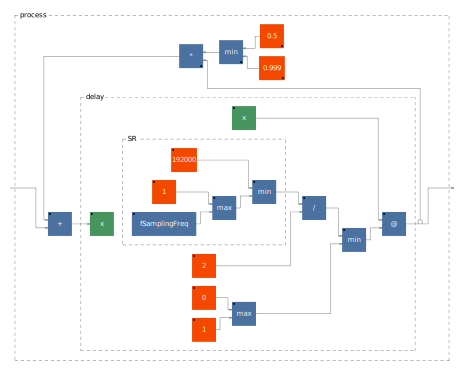
\includegraphics[width=\textwidth]{CAPITOLI/0500/CODES/REV/dfl-svg/process.pdf}
  \caption[]{Delay in Feedback Loop. Implementazione Faust.}
  \label{faust:dfl}
\end{figure}

Il primo oggetto che Schroeder descrive è quindi una linea di ritardo
alimentata da un circuito di retroazione controllato dal coefficiente $g < 1$.

Il filtro prevede un valore di ritardo $t$ applicato a tutti i campioni in
entrata, situazione che può avere diversi significati, come cercherò di spiegare
in seguito.

Il codice Faust per la realizzazione di tale oggetto è il seguente.

\lstinputlisting{CAPITOLI/0500/CODES/REV/dfl.dsp}

Il codice di descrizione della funzione è presente tutto in riga tre, la quale
può essere smontata in più parti per comprenderne la sintassi.

Il blocco di ritardo \texttt{delay} deve essere inizializzato con l'allocazione
di memoria massima in campioni. L'impostazione inserita \texttt{SR/2} permette
di avere almeno mezzo secondo a qualsiasi requenza di campionamento. Il tempo
$t$ di ritardo effettivo, in quanto unità al campione, deve essere necessariamente
un intero, motivo per cui la variabile in entrata $t$ viene passata per una
funzione \texttt{int} che ne scarta eventuali valori decimali.

L'uscita del blocco di ritardo viene prelevata prima dell'uscita dal filtro e
reindirizzata alla sua entrata, adeguatamente scalata dal coeffficiente $g < 1$,
in somma con l'entrata del filtro.

\begin{figure}[ht]
  \centering
  \includegraphics[width=\textwidth]{CAPITOLI/0500/IMG/dfl-ir.png}
  \caption[]{Schroeder dfl impulse response.}
  \label{schroeder:dflir}
\end{figure}

Schoreder fornisce una chiara descrizione del funzionamento temporale del filtro
ed attraverso un diagramma ne mostra la risposta all'impulso. La figura
\ref{schroeder:dflir} mostra il comportamento del filtro ad un tempo $t$
consistente in ripetizioni successive per multipli interi $2t$, $3t$ \ldots fino
al completo esaurimento dell'ampiezza per opera del coefficiente scalare $g$.

\begin{figure}[ht]
  \centering
  \includegraphics[width=\textwidth]{CAPITOLI/0500/CODES/REV/dfl.png}
  \caption[]{Faust dfl impulse response.}
  \label{faust:dflir}
\end{figure}

La risposta all'impulso illustrata in figura \ref{schroeder:dflir} indica un
decadimento esponenziale per ogni riflessione eco.

Possiamo descrivere allo stesso modo il nostro modello: il tempo di ritardo $t$
regola le nuove occorrenze dell'impulso generate dal circuito di retroazione
scalate dal coefficiente $g$. Pur avendo creato un modello di filtro
apparentemente identico, producente un diagramma a blocchi \ref{faust:dfl}
piuttosto fedele al modello di Schroeder, la risposta all'impulso del nostro
filtro si comporta in modo diverso, motivo per cui merita uno sguardo di analisi
e un'attenta riflessione.

La risposta all'impulso di figura \ref{faust:dflir} è stata generata impostando
le variabili $t=1$ (un campione di ritardo) e $g=0.5$ (ampiezza dimezzata ad
ogni giro di feedback). Ci si aspetta quindi un comportamento molto simile a
quello descritto da Schroeder, per una successione di multipli di $1$ dovremmo
avere il primo impulso nella posizione $n[1]$ con ampiezza $a=1$ (non scalata,
non l'impulso non è ancor transitato nel ciclo di ffeedback). Il secondo impulso
dovrebbe essere posizionato subito dopo il primo, nella posizione $n[2]$ con
ampiezza $a=0.5$, e cosi proseguendo. Tuttavia, osservando l'indicizzazione dei
campioni sull'asse delle ascisse della figura \ref{faust:dflir} si può constatare
che in realtà il nostro filtro sta impiegando due campioni per ogni ciclo
impulsivo in luogo di uno, posizionando gli impulsi per $2t$.

La motivazione di questa differenza è nascosta dietro al significato del diagramma
a blocchi di entrambe le rappresentazioni. Nella prima, quella originaria di Schroeder,
il punto di prelievo del segnale per il ciclo di feedback è a tempo zero, ovvero
linea che porta il segnale dall'uscita del blocco di ritardo all'entrata della
somma è istantanea. Nella descrizione algoritmica di faust mediante diagramma
a blocchi invece l'operatore $~$ produce contestualmente al prelievo del segnale,
un inevitabile campione di ritardo. La linea di ricircolo quindi, nel momento
in cui alimenta il blocco di ritardo, porta già un campione di ritardo su quello
corrente.

La correzione di questo filtro per ottenere il comportamento prospettato da Schroeder
consiste nel sottrarre il campione di ritardo, prodotto dalla ricorsione, alla
variabile $t$ con $t-1$. Questo tipo di intervento per $t=$ produrrà $t=1-1=0$
ovvero zero campioni di ritardo all'uscita, un campione, come richiesto,
scalato in $g$ all'entrata della somma di ricircolo. Questo tipo di operazione
crea però un offset temporale in quanto la sequenza di campioni ritardati, ora
corretta, si trova in uscita un campione prima (ritardo zero) di quello richiesto.
Anche questa problematica è risolvibile inserendo un ulteriore campione di ritardo
\texttt{mem} all'uscita dell'algoritmo, in modo da bilanciare l'intera sequenza
temporale.

\lstinputlisting{CAPITOLI/0500/CODES/REV/dflc.dsp}

La risposta all'impulso del filto corretto è ora coerente con le aspettative.

\begin{figure}[ht]
  \centering
  \includegraphics[width=\textwidth]{CAPITOLI/0500/CODES/REV/dflc.png}
  \caption[]{Faust dfl impulse response.}
  \label{faust:dflir}
\end{figure}

Il filtro appena costruito può operare tempi di ritardo tra $1$ e \emph{Nyquist}.
Questo comportamento può portare a diversi risultati sonori, dal più diretto
ritardo di una quantità di campioni indicata con $g=0$, oppure ad un filtraggio di componenti
spettrali in funzione di $t$ e $g$.

\begin{figure}[h]
  \centering
  \includegraphics[width=\textwidth]{CAPITOLI/0500/IMG/dfl-fr.png}
  \caption[]{Schroeder dfl risposta in requenza, \emph{”somigliante ad un pettine”}.}
  \label{schroeder:dflffr}
\end{figure}

\begin{quote}
  The amplitude-frequency responce has the appearance of a comb with periodic
  maxima and minima\ldots It is these peaks and valleyys which impart the undesidered
  “colored” qualityy to sound reverberated by devices like that.
\end{quote}

Il rapporto tra la risposta massima e quella minima è espresso dalla formula:

\begin{equation}
  \label{comb-filter}
  H_{max}/H_{min} = (1+g)/(1-g)
\end{equation}

il che porta a considerare che per un coefficiente $g=0.708$ corrispondente ad
un abbattimento di $-3dB$ il rapporto di di $5.849:1$ (espresso da $1.708/0.292$)

\begin{equation}
  \label{hmax}
  \Delta_{amp} = 20\times Log_10(5.849) = 15.34 dB
\end{equation}

ovvero $15.34dB$ di escursione.

\begin{quote}
  In a search for better artificial reverberators\ldots (we) noted that certain
  mixture of the output of the multiply delayed sound and the undelayed sound
  would result in an equal response of the reverberator for all frequencies.
\end{quote}

Questo passo è cruciale per comprendere il processo evolutivo dei meccanismi
riverberanti di Schroeder. Il filtro IIR passa da un campione di ritardo (passa
basso) ad un delay variabile (comb-filter) e sta per diventare un filtro
lineare in frequenza (all-pass) attraverso una oculata gestione dei rapporto tra
suono diretto e suono ritardato. La proporzione per contenere l'energia unitaria
su tutto lo spettro di frequenze è $-g$ per il segnale diretto e $1-g^2$
per il segnale ritardato.

\begin{figure}[ht]
  \centering
  \includegraphics[width=\textwidth]{CAPITOLI/0500/IMG/allpass.png}
  \caption[]{All-pass, diagramma a blocchi e risposta all'impulso.}
  \label{schroeder:allpass}
\end{figure}

\begin{quote}
  \ldots the addition of a suitably proportioned uunudelayyed path has converted
  the comb-filter (fig. \ref{schroeder:dfl}) into an all-pass (fig.
  \ref{schroeder:allpass}). This is not a mere academic result.
\end{quote}

Il filtro all-pass ora permette di passare tutte le frequenze con eguale ampiezza
e senza “colorare” il segnale. Si possono connettere tra loro diverse unità di
questo tipo per raggiungere la densità di eco necessaria. Inoltre il filtro
all-pass condivide con i filtri comb le proprietà del feedback e del decadimento
esponenziale dell'energia, lo stesso comportamento che si presenta nelle buone
situazioni acustiche.

\lstinputlisting{CAPITOLI/0500/CODES/REV/apf.dsp}

\printbibliography
\end{refsection}
